\documentclass[12pt,letterpaper]{article}
\usepackage[spanish,es-nodecimaldot]{babel}
\usepackage[utf8]{inputenc}
\usepackage[T1]{fontenc}
\usepackage{geometry}
\usepackage{graphicx}
\usepackage{amsmath,amssymb}
\usepackage{booktabs}
\usepackage{float}
\usepackage{array}
\usepackage{longtable}
\geometry{margin=2.3cm}
\graphicspath{{figuras/}}

\title{Explicación detallada de LightGBM optimizado con Optuna y de la trayectoria Monte Carlo del oro}
\author{Alejandro Ramirez \and Leidy Paola Patiño}
\date{\today}

\begin{document}
\maketitle

\section{Propósito}
Este documento explica de forma detallada el modelo final utilizado en el proyecto: \textbf{LightGBM optimizado con Optuna}. También se muestra cómo se construye una trayectoria Monte Carlo desde el primer día simulado hasta el valor final. La idea es dejar claro qué hace el modelo, qué variables usa, cómo funcionan los árboles, qué optimiza Optuna y por qué la simulación entregó los valores observados.

\section{Qué es LightGBM}
LightGBM significa \textit{Light Gradient Boosting Machine}. Es una librería de aprendizaje automático para construir modelos predictivos basados en árboles de decisión y \textit{gradient boosting}. Es ampliamente usada en datos tabulares, predicción financiera, riesgo, precios, demanda, clasificación y regresión.

En este trabajo LightGBM se usó para resolver una tarea de regresión: estimar el log-retorno del precio del oro del siguiente día hábil. No se predijo directamente el precio, sino el retorno logarítmico:
\begin{equation}
r_{t+1}=\ln\left(\frac{P_{t+1}}{P_t}\right),
\end{equation}
donde $P_t$ es el precio del oro en el día actual y $P_{t+1}$ el precio del siguiente día hábil.

Luego, el precio se reconstruyó con:
\begin{equation}
\hat{P}_{t+1}=P_t e^{\hat{r}_{t+1}}.
\end{equation}

Esta formulación es útil porque los retornos suelen ser más estables que los precios en nivel. Además, evita que el modelo aprenda directamente una tendencia de precio sin entender los cambios relativos.

\section{Cómo funcionan los árboles de decisión}
Un árbol de decisión divide los datos mediante reglas. Cada regla pregunta si una variable cumple una condición:
\begin{equation}
x_j \leq c,
\end{equation}
donde $x_j$ es una variable explicativa y $c$ es un punto de corte.

Por ejemplo, una rama puede preguntar:
\begin{equation}
\text{volatilidad\_oro\_5} \leq c_1.
\end{equation}
Si la respuesta es sí, la observación va a la rama izquierda; si no, va a la rama derecha. Más adelante el árbol puede preguntar por otra variable, por ejemplo:
\begin{equation}
\text{retorno\_plata\_5} \leq c_2.
\end{equation}

Al final de cada camino hay una hoja. Esa hoja contiene un valor numérico que se suma a la predicción del retorno. En un modelo de boosting no hay un solo árbol, sino muchos árboles pequeños que se suman entre sí.

\section{Cómo funciona el Gradient Boosting}
LightGBM construye árboles de forma secuencial. Cada árbol nuevo intenta corregir los errores de los árboles anteriores. La predicción final del retorno se puede expresar así:
\begin{equation}
\hat{r}_{t+1}=F_M(X_t)=F_0(X_t)+\eta\sum_{m=1}^{M} f_m(X_t),
\end{equation}
donde:
\begin{itemize}
    \item $X_t$ es el vector de variables disponibles en el día $t$.
    \item $F_0$ es una predicción inicial.
    \item $f_m$ es el árbol número $m$.
    \item $M$ es el número de árboles.
    \item $\eta$ es el \textit{learning rate} o tasa de aprendizaje.
\end{itemize}

La lógica es:
\begin{enumerate}
    \item El modelo empieza con una predicción inicial.
    \item Calcula cuánto se equivocó.
    \item Entrena un árbol para corregir ese error.
    \item Agrega ese árbol con peso pequeño.
    \item Repite el proceso muchas veces.
\end{enumerate}

LightGBM usa crecimiento por hojas, conocido como \textit{leaf-wise growth}. Esto quiere decir que no divide todos los niveles del árbol al mismo tiempo, sino que busca la hoja donde más puede reducir el error. Esto suele mejorar la precisión, pero por eso se controlan hiperparámetros como \texttt{num\_leaves} y \texttt{min\_child\_samples}.

\section{Qué es Optuna}
Optuna es una librería de optimización automática de hiperparámetros. Un hiperparámetro es una decisión de diseño del modelo, por ejemplo cuántos árboles usar, qué tasa de aprendizaje usar o cuántas hojas puede tener cada árbol.

Optuna hizo lo siguiente:
\begin{enumerate}
    \item Propuso una combinación de hiperparámetros.
    \item Entrenó LightGBM con esa combinación.
    \item Midió el error usando validación temporal.
    \item Guardó el RMSE promedio.
    \item Propuso una nueva combinación, aprendiendo de las anteriores.
\end{enumerate}

El objetivo matemático fue minimizar el error RMSE promedio en validación temporal:
\begin{equation}
\min_{\theta} RMSE_{CV}(\theta),
\end{equation}
donde $\theta$ representa los hiperparámetros.

La configuración ganadora fue:
\begin{table}[H]
\centering
\caption{Hiperparámetros finales de LightGBM encontrados por Optuna.}
\begin{tabular}{lrp{7.5cm}}
\toprule
Hiperparámetro & Valor & Interpretación \\
\midrule
\texttt{n\_estimators} & 400 & Número de árboles construidos por el modelo. \\
\texttt{learning\_rate} & 0.0174355 & Peso de cada árbol nuevo. Un valor bajo hace que el aprendizaje sea gradual. \\
\texttt{num\_leaves} & 38 & Número máximo de hojas por árbol. Controla la complejidad de las reglas. \\
\texttt{subsample} & 0.810038 & Proporción de observaciones usadas en cada árbol. \\
\texttt{colsample\_bytree} & 0.730510 & Proporción de variables usadas por árbol. \\
\texttt{min\_child\_samples} & 23 & Mínimo de observaciones necesarias en una hoja. \\
\bottomrule
\end{tabular}
\end{table}

\section{Todas las variables usadas por el modelo}
El modelo final usó 76 variables. La Tabla \ref{tab:todasvariables} las agrupa por tipo y explica qué información aportan.

\begin{longtable}{p{4.2cm}p{10.2cm}}
\caption{Variables usadas por LightGBM.}\label{tab:todasvariables}\\
\toprule
Variable & Significado \\
\midrule
\endfirsthead
\toprule
Variable & Significado \\
\midrule
\endhead
precio\_oro & Precio actual del oro en USD/oz. \\
precio\_plata & Precio actual de la plata en USD/oz. \\
ni\_precio\_recursos & Precio de oro usado para recursos minerales en reportes NI 43-101. \\
ni\_precio\_reservas & Precio de oro usado para reservas minerales en reportes NI 43-101. \\
cpi\_us & Índice de precios al consumidor de Estados Unidos disponible. \\
fed\_funds & Tasa de fondos federales disponible. \\
sp500 & Nivel del índice S\&P 500 disponible. \\
retorno\_oro\_1 & Retorno porcentual del oro a 1 día. \\
retorno\_oro\_5 & Retorno porcentual del oro a 5 días. \\
retorno\_oro\_10 & Retorno porcentual del oro a 10 días. \\
diferencia\_oro\_1 & Diferencia del precio del oro frente al día anterior. \\
diferencia\_oro\_5 & Diferencia del precio del oro frente a 5 días atrás. \\
diferencia\_oro\_10 & Diferencia del precio del oro frente a 10 días atrás. \\
precio\_oro\_lag\_1 & Precio del oro con rezago de 1 día. \\
precio\_oro\_lag\_2 & Precio del oro con rezago de 2 días. \\
precio\_oro\_lag\_3 & Precio del oro con rezago de 3 días. \\
precio\_oro\_lag\_5 & Precio del oro con rezago de 5 días. \\
precio\_oro\_lag\_10 & Precio del oro con rezago de 10 días. \\
precio\_oro\_lag\_20 & Precio del oro con rezago de 20 días. \\
ma\_oro\_3 & Media móvil simple del oro a 3 días. \\
ema\_oro\_3 & Media móvil exponencial del oro a 3 días. \\
volatilidad\_oro\_3 & Volatilidad móvil del oro a 3 días. \\
ma\_oro\_5 & Media móvil simple del oro a 5 días. \\
ema\_oro\_5 & Media móvil exponencial del oro a 5 días. \\
volatilidad\_oro\_5 & Volatilidad móvil del oro a 5 días. \\
ma\_oro\_10 & Media móvil simple del oro a 10 días. \\
ema\_oro\_10 & Media móvil exponencial del oro a 10 días. \\
volatilidad\_oro\_10 & Volatilidad móvil del oro a 10 días. \\
ma\_oro\_20 & Media móvil simple del oro a 20 días. \\
ema\_oro\_20 & Media móvil exponencial del oro a 20 días. \\
volatilidad\_oro\_20 & Volatilidad móvil del oro a 20 días. \\
ma\_oro\_30 & Media móvil simple del oro a 30 días. \\
ema\_oro\_30 & Media móvil exponencial del oro a 30 días. \\
volatilidad\_oro\_30 & Volatilidad móvil del oro a 30 días. \\
ratio\_oro\_plata & Relación entre precio del oro y precio de la plata. \\
retorno\_plata\_1 & Retorno porcentual de la plata a 1 día. \\
retorno\_plata\_5 & Retorno porcentual de la plata a 5 días. \\
diferencia\_plata\_1 & Diferencia diaria del precio de la plata. \\
precio\_plata\_lag\_1 & Precio de la plata con rezago de 1 día. \\
precio\_plata\_lag\_2 & Precio de la plata con rezago de 2 días. \\
precio\_plata\_lag\_5 & Precio de la plata con rezago de 5 días. \\
precio\_plata\_lag\_10 & Precio de la plata con rezago de 10 días. \\
ma\_plata\_5 & Media móvil simple de la plata a 5 días. \\
volatilidad\_plata\_5 & Volatilidad móvil de la plata a 5 días. \\
ma\_plata\_10 & Media móvil simple de la plata a 10 días. \\
volatilidad\_plata\_10 & Volatilidad móvil de la plata a 10 días. \\
ma\_plata\_20 & Media móvil simple de la plata a 20 días. \\
volatilidad\_plata\_20 & Volatilidad móvil de la plata a 20 días. \\
cpi\_us\_chg\_1 & Cambio porcentual de CPI a 1 periodo. \\
cpi\_us\_chg\_5 & Cambio porcentual de CPI a 5 periodos. \\
cpi\_us\_lag\_1 & CPI rezagado 1 periodo. \\
cpi\_us\_ma\_5 & Media móvil de CPI a 5 periodos. \\
cpi\_us\_ma\_20 & Media móvil de CPI a 20 periodos. \\
fed\_funds\_chg\_1 & Cambio porcentual de fed funds a 1 periodo. \\
fed\_funds\_chg\_5 & Cambio porcentual de fed funds a 5 periodos. \\
fed\_funds\_lag\_1 & Fed funds rezagado 1 periodo. \\
fed\_funds\_ma\_5 & Media móvil de fed funds a 5 periodos. \\
fed\_funds\_ma\_20 & Media móvil de fed funds a 20 periodos. \\
sp500\_chg\_1 & Cambio porcentual del S\&P 500 a 1 día. \\
sp500\_chg\_5 & Cambio porcentual del S\&P 500 a 5 días. \\
sp500\_lag\_1 & S\&P 500 rezagado 1 día. \\
sp500\_ma\_5 & Media móvil del S\&P 500 a 5 días. \\
sp500\_ma\_20 & Media móvil del S\&P 500 a 20 días. \\
ni\_gap\_recursos\_reservas & Diferencia entre precio NI de recursos y precio NI de reservas. \\
anio & Año calendario. \\
mes & Mes calendario. \\
trimestre & Trimestre calendario. \\
dia\_mes & Día del mes. \\
dia\_semana & Día de la semana. \\
semana\_anio & Semana del año. \\
mes\_inicio & Indicador de inicio de mes. \\
mes\_fin & Indicador de fin de mes. \\
mes\_sin & Componente seno del ciclo mensual. \\
mes\_cos & Componente coseno del ciclo mensual. \\
dia\_semana\_sin & Componente seno del ciclo semanal. \\
dia\_semana\_cos & Componente coseno del ciclo semanal. \\
\bottomrule
\end{longtable}

\section{Variables más usadas en las decisiones de los árboles}
Aunque el modelo recibió 76 variables, unas tuvieron más peso en las divisiones de los árboles. Las principales fueron:
\begin{table}[H]
\centering
\caption{Variables con mayor importancia en LightGBM.}
\begin{tabular}{lr}
\toprule
Variable & Importancia \\
\midrule
volatilidad\_oro\_5 & 619 \\
retorno\_plata\_5 & 607 \\
volatilidad\_oro\_3 & 606 \\
retorno\_oro\_5 & 592 \\
volatilidad\_oro\_10 & 584 \\
sp500\_chg\_1 & 577 \\
volatilidad\_plata\_10 & 562 \\
diferencia\_oro\_5 & 518 \\
volatilidad\_oro\_30 & 517 \\
sp500\_chg\_5 & 516 \\
\bottomrule
\end{tabular}
\end{table}

\begin{figure}[H]
\centering
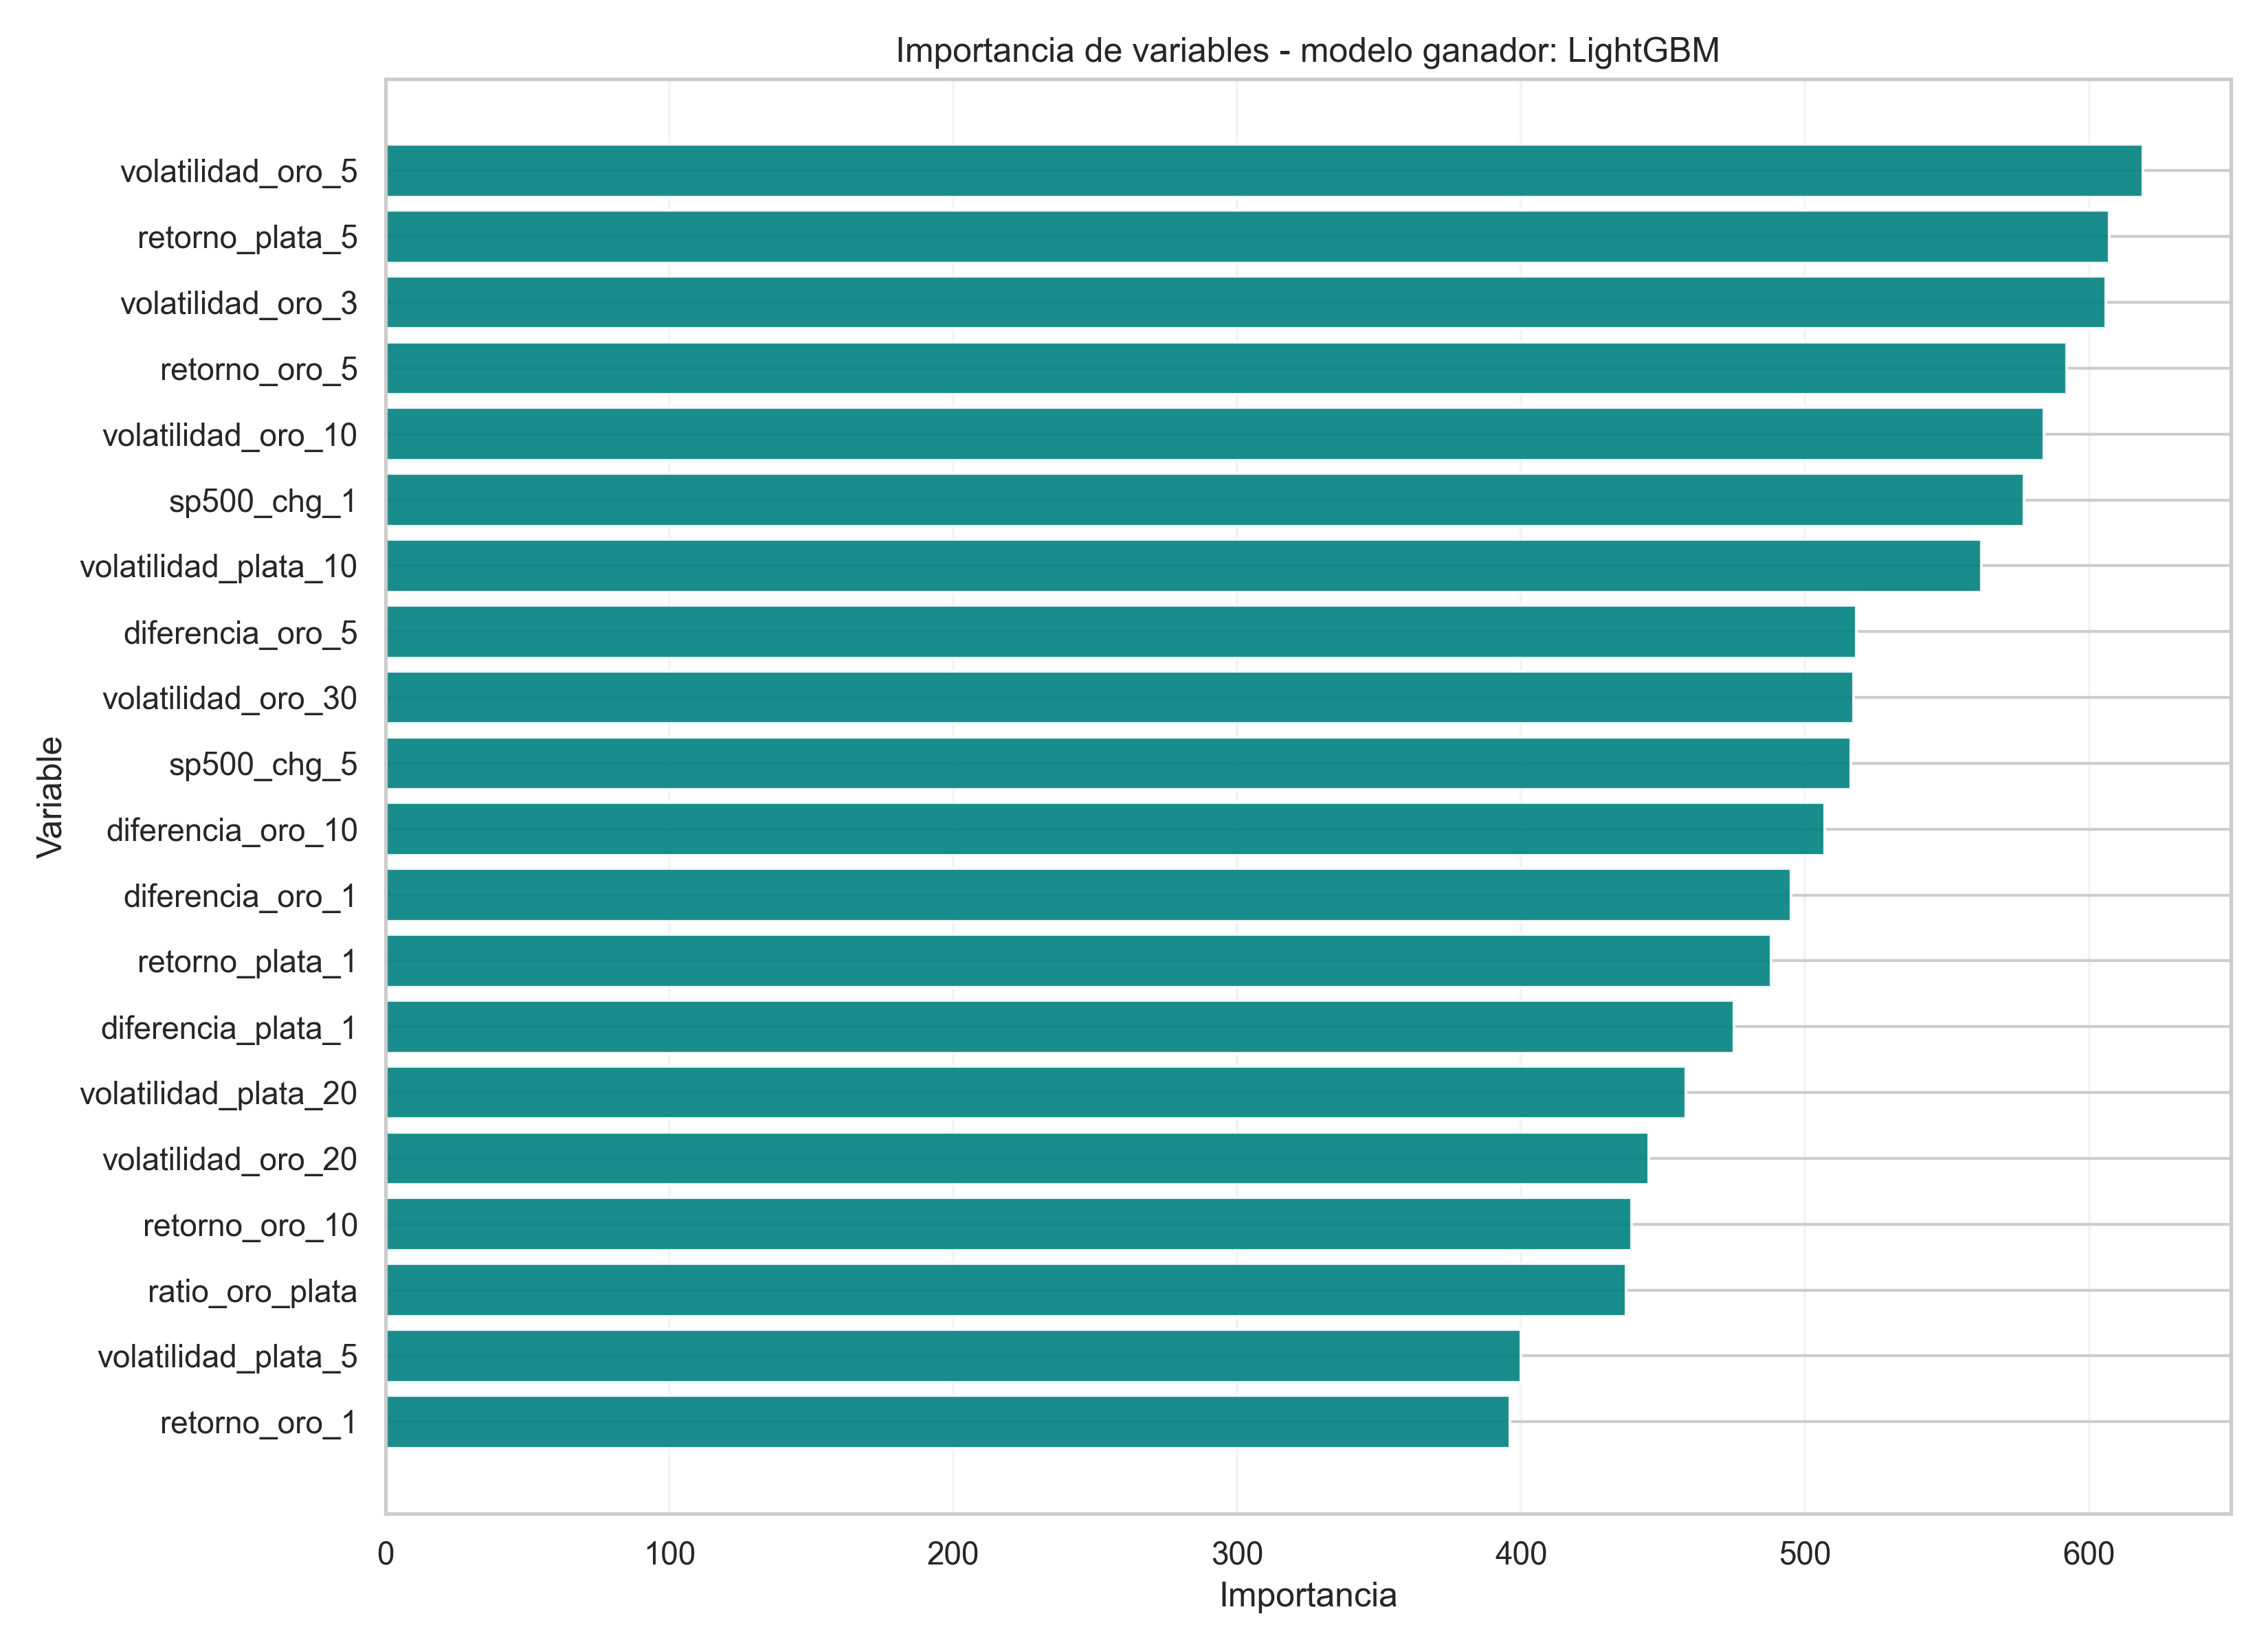
\includegraphics[width=0.95\textwidth]{04_importancia_variables.png}
\caption{Importancia de variables del modelo LightGBM seleccionado.}
\end{figure}

\section{Por qué LightGBM fue el modelo final}
El modelo final fue seleccionado porque tuvo el menor RMSE promedio en validación temporal. La comparación principal fue:
\begin{table}[H]
\centering
\caption{Comparación por validación temporal.}
\begin{tabular}{lrrr}
\toprule
Modelo & MAE CV & RMSE CV & $R^2$ CV \\
\midrule
LightGBM + Optuna & 17.4113 & 22.5191 & 0.9669 \\
LightGBM manual & 18.1269 & 23.4337 & 0.9639 \\
HistGradientBoosting & 18.8968 & 24.3490 & 0.9633 \\
CatBoost & 19.0538 & 24.3956 & 0.9663 \\
XGBoost & 21.4520 & 27.7745 & 0.9575 \\
\bottomrule
\end{tabular}
\end{table}

Esto significa que XGBoost fue superado en esta versión mejorada, aunque había sido el mejor en el trabajo anterior.

\section{Cómo se genera una trayectoria Monte Carlo}
El modelo LightGBM entrega un retorno base para cada día futuro:
\begin{equation}
\hat{r}_t=f(X_t).
\end{equation}
Luego la simulación Monte Carlo agrega un choque aleatorio:
\begin{equation}
r_t^{MC}=\hat{r}_t+\text{choque}_t.
\end{equation}
Ese choque viene de la volatilidad histórica/residual y de la estructura aleatoria del escenario base. Por eso la simulación ``botó'' un valor distinto a la mediana: no usa solo el retorno esperado del modelo, sino que agrega incertidumbre.

Después se reemplaza el retorno simulado en la fórmula exponencial:
\begin{equation}
P_t^{MC}=P_{t-1}^{MC}e^{r_t^{MC}}.
\end{equation}

La fórmula acumulada desde el inicio hasta cualquier fecha $T$ es:
\begin{equation}
P_T^{MC}=P_0\exp\left(\sum_{t=1}^{T}r_t^{MC}\right).
\end{equation}

\section{Ejemplo numérico paso a paso}
La trayectoria inicia con el último precio histórico observado:
\begin{equation}
P_0=4719.285\;\text{USD/oz}.
\end{equation}

\subsection{Primer día simulado: 2026-04-09}
El modelo LightGBM entregó un retorno base:
\begin{equation}
\hat{r}_1=0.001800.
\end{equation}
La simulación Monte Carlo generó un choque negativo:
\begin{equation}
\text{choque}_1=-0.018433.
\end{equation}
Entonces el retorno simulado fue:
\begin{equation}
r_1^{MC}=0.001800-0.018433=-0.016633.
\end{equation}
Se reemplaza en la fórmula:
\begin{equation}
P_1^{MC}=4719.285\times e^{-0.016633}=4641.44\;\text{USD/oz}.
\end{equation}
La simulación entregó un precio menor porque el choque aleatorio fue negativo y superó al retorno base positivo del modelo.

\subsection{Segundo día simulado: 2026-04-10}
Ahora el precio inicial ya no es 4719.285, sino el precio simulado anterior:
\begin{equation}
P_1^{MC}=4641.44.
\end{equation}
El retorno base fue nuevamente 0.001800 y el choque fue 0.000488:
\begin{equation}
r_2^{MC}=0.001800+0.000488=0.002288.
\end{equation}
Entonces:
\begin{equation}
P_2^{MC}=4641.44\times e^{0.002288}=4652.07\;\text{USD/oz}.
\end{equation}

\subsection{Tercer día simulado: 2026-04-13}
El retorno simulado fue:
\begin{equation}
r_3^{MC}=0.001800+0.021479=0.023279.
\end{equation}
Por tanto:
\begin{equation}
P_3^{MC}=4652.07\times e^{0.023279}=4761.64\;\text{USD/oz}.
\end{equation}
Aquí la trayectoria subió porque el choque fue fuerte y positivo.

\subsection{Primeros pasos resumidos}
\begin{table}[H]
\centering
\caption{Primeros valores de la trayectoria Monte Carlo.}
\begin{tabular}{lrrrr}
\toprule
Fecha & Retorno base & Choque & Retorno MC & Precio MC \\
\midrule
2026-04-09 & 0.001800 & -0.018433 & -0.016633 & 4641.44 \\
2026-04-10 & 0.001800 & 0.000488 & 0.002288 & 4652.07 \\
2026-04-13 & 0.001800 & 0.021479 & 0.023279 & 4761.64 \\
2026-04-14 & 0.001800 & 0.014592 & 0.016392 & 4840.34 \\
2026-04-15 & 0.000951 & 0.012809 & 0.013761 & 4907.40 \\
\bottomrule
\end{tabular}
\end{table}

\section{Cómo se llega al resultado final}
La trayectoria tiene 2538 pasos, desde 2026-04-09 hasta 2035-12-31. En cada paso se repite exactamente el mismo procedimiento:
\begin{enumerate}
    \item LightGBM calcula $\hat{r}_t$ usando las 76 variables disponibles o proyectadas.
    \item Monte Carlo genera un choque $\text{choque}_t$.
    \item Se calcula $r_t^{MC}=\hat{r}_t+\text{choque}_t$.
    \item Se actualiza el precio con $P_t=P_{t-1}e^{r_t^{MC}}$.
\end{enumerate}

Para no imprimir 2538 operaciones una por una, se usa la forma acumulada. La suma de todos los retornos simulados de la trayectoria fue:
\begin{equation}
\sum_{t=1}^{2538}r_t^{MC}=0.735430.
\end{equation}
Entonces el precio final se obtiene reemplazando en la fórmula acumulada:
\begin{equation}
P_{2538}^{MC}=4719.285\times e^{0.735430}=9846.22\;\text{USD/oz}.
\end{equation}

Ese es el valor final de la trayectoria individual en 2035-12-31. No es la mediana del escenario, sino una ruta posible. La mediana $P50$ del escenario base para esa fecha fue 5427.87 USD/oz, mientras que esta trayectoria terminó más arriba porque la suma acumulada de choques fue positiva.

\subsection{Últimos pasos de la trayectoria}
\begin{table}[H]
\centering
\caption{Últimos valores de la trayectoria Monte Carlo.}
\begin{tabular}{lrrrr}
\toprule
Fecha & Retorno base & Choque & Retorno MC & Precio MC \\
\midrule
2035-12-25 & -0.000050 & -0.005057 & -0.005107 & 9356.17 \\
2035-12-26 & -0.000050 & -0.014985 & -0.015035 & 9216.55 \\
2035-12-27 & -0.000050 & 0.003705 & 0.003655 & 9250.30 \\
2035-12-28 & 0.001185 & 0.020016 & 0.021201 & 9448.51 \\
2035-12-31 & -0.000050 & 0.041281 & 0.041231 & 9846.22 \\
\bottomrule
\end{tabular}
\end{table}

\section{Lectura de la gráfica}
En la Figura \ref{fig:trayectoria}, la línea roja es la trayectoria individual calculada con los pasos anteriores. La línea naranja es la mediana $P50$ del escenario base y la banda sombreada representa los percentiles $P10$ y $P90$.

\begin{figure}[H]
\centering
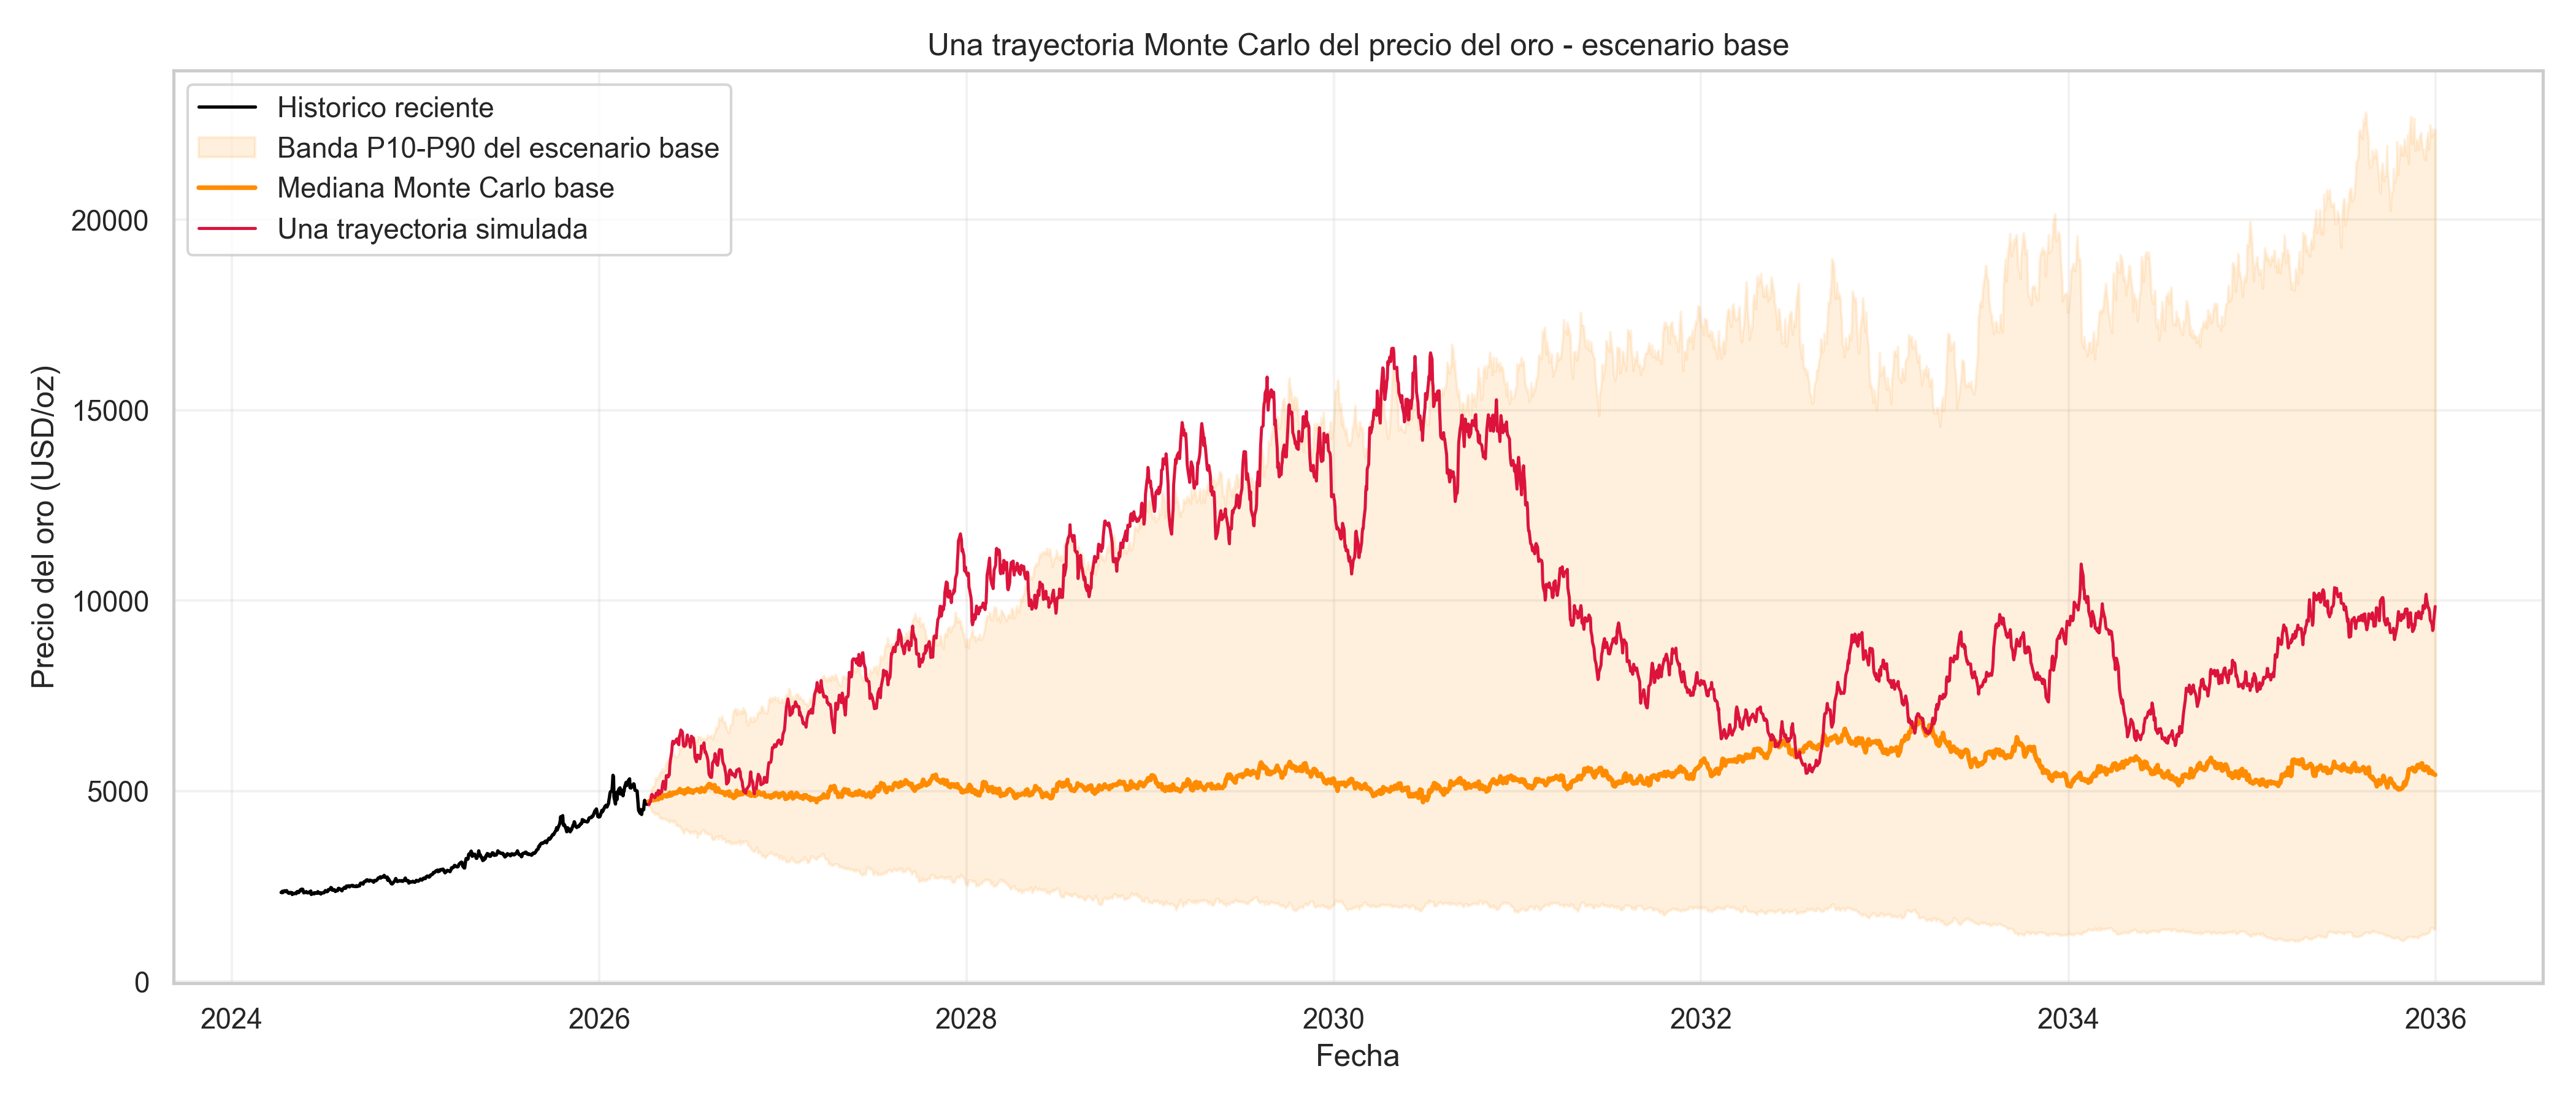
\includegraphics[width=0.95\textwidth]{09_trayectoria_unica_monte_carlo_base.png}
\caption{Trayectoria individual generada con LightGBM + Optuna y Monte Carlo.}
\label{fig:trayectoria}
\end{figure}

Si la línea roja sube por encima de la mediana, significa que los choques acumulados de esa ruta fueron más positivos que el caso central. Si se acerca al percentil 90, está en la parte alta de la distribución simulada. Si baja hacia el percentil 10, está en la parte baja.

\section{Conclusión}
LightGBM + Optuna funciona combinando árboles de decisión secuenciales con búsqueda automática de hiperparámetros. Los árboles deciden usando variables como volatilidad del oro, retornos de la plata, diferencias del oro y cambios del S\&P 500. Optuna encontró una configuración que redujo el RMSE de validación temporal frente a XGBoost y otros modelos. Luego, la trayectoria Monte Carlo tomó los retornos base de LightGBM, agregó choques aleatorios y actualizó el precio día a día con la fórmula exponencial. Por eso cada valor de la trayectoria tiene una explicación: proviene de un retorno base del modelo más un choque de simulación, reemplazado en $P_t=P_{t-1}e^{r_t}$.

\end{document}
